\chapter{Comparison to Other Models}
It is well known that Black-Scholes model assumes constant volatility which is not realistic in real market. Using Exploratory Data Analysis (EDA) techniques, we visualized the volatility data in Bloomberg Terminal and presented following figures. 

\begin{figure}[htb]
	\centering
	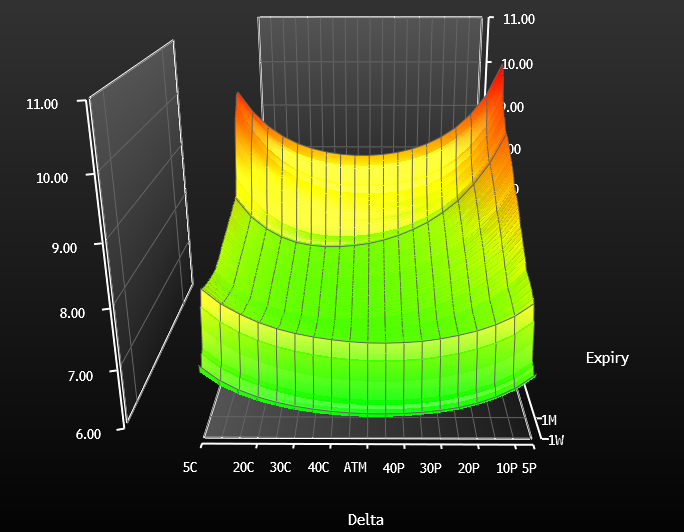
\includegraphics[scale=0.8]{./Testing-data/Heston-prices/VolSurface/EURUSD-Vol.png} 
	\caption{Three-dimensional volatility surface in terms of Delta and Maturity Time for EUR/USD option, observed on May 10, 2017. Source: \textit{Bloomberg}}
	\label{fig:3dvol-label} % insert suitable label, this is used to refer to a fig from within the text as shown above
\end{figure}
\begin{figure}[htb]
	\centering
	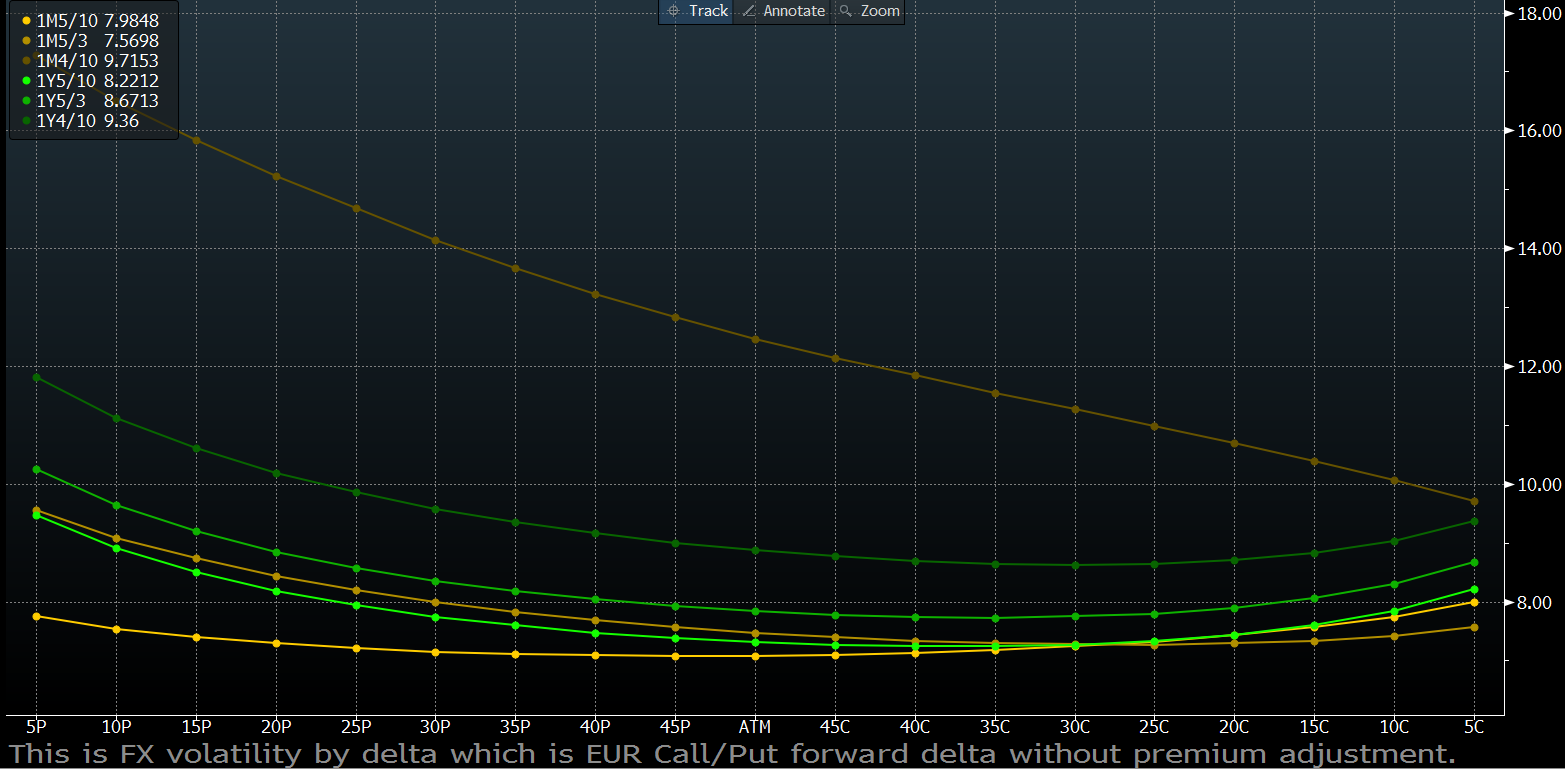
\includegraphics[scale=0.415]{./Testing-data//Heston-prices/VolSurface/EURUSD-2DVol.png} 
	\caption{Volatility surface in terms of Delta for 1-month and 1-year EUR/USD option. Source: \textit{Bloomberg}}
	\label{fig:2dvol-label} % insert suitable label, this is used to refer to a fig from within the text as shown above
\end{figure}
\noindent
From both figures we clearly see that the volatility is not constant. Figure 5.1 shows three-dimensional volatility surface for EUR/USD option. Consider a given expiration, deep in-the-money and out-of-the money options have higher implied volatility than at-the-money option. If we fix a specific strike, we could obtained that long-term maturity usually has higher implied volatility.\newline\newline
In Figure 5.2 we selected 1-month and 1-year EUR/USD option and showed the volatility change in terms of Delta. For 1-month option  data extracted on Apr. 10, 2017, volatility skew was observed while volatility smile detected for other dates.
\newline\newline
In addition to the simplified Vanna-Volga method we introduced in Chapter 3, several other models have been developed to mitigate the volatility smile impact. Here we will briefly introduce the exact Vanna-Volga pricing method and two stochastic volatility model: Heston model and SABR model.

\section{The Exact Vanna-Volga Method}
As mentioned, the simplified method is a good approximation while neglecting some small fraction of Vanna and Volga. A modified Vanna-Volga method, which provide more accurate result, has been proposed (e.g. Carr et al. (2006), Fisher (2007)) and proved (Shkolnikov (2009)). It has been shown that the following proposition is true for any contract.
\begin{prop}
	Under the assumption that $S$ follows Geometric Brownian motion with stochastic but strike-independent implied volatility, there exists a unique self-financing portfolio $\Pi^{MK} = X^{MK}-\Delta^{MK} S-\sum_{i=1}^{3}x_i C_i^{MK}$ such that $\Pi^{MK} = \Pi^{BS}$ for any $0 \leq t \leq T$. It follows that the Vanna-Volga price is given by:
	\begin{align}
	X_{VV} = X^{BS}+\sum_{i=1}^{3}x_i\left( C_i - C_{i}^{BS}\right) 
	\end{align}
\end{prop}
It is worth noting that in the exact formula, the pivot calls and pivot puts could be used interchangeably due to the put-call parity. Using puts would change the value of delta but the coefficient vector $x_i$ would not be affected. \newline

\section{Heston Model}
The Heston Model is a commonly used stochastic volatility model, in which the randomness of the variance process varies as the square root of variance.
\newline\newline
In basic Heston model, the underlying asset $S_t$ follows a stochastic process:
\begin{align}
dS_t = \mu S_t dt + \sqrt{\nu_t}S_tdW_{t}^S
\end{align}
where the instantaneous variance $\nu_t$ is a CIR process:
\begin{align}
d\nu_t = \kappa\left( \theta - \nu_t\right)  dt + \xi \sqrt{\nu_t}dW_{t}^{\nu}
\end{align}
and $dW_{t}^S$, $dW_{t}^{\nu}$ are Wiener processes with correlation $\rho$.
\newline\newline
The parameters have following meanings:
\begin{itemize}
	\item $\mu$ is the rate of return of the asset.
	\item $\kappa$ is the mean reversion speed.
	\item $\theta$ is the long term average price variance.
	\item $\xi$ is the volatility of volatility which determines the variance of $\nu_t$.
\end{itemize}
The Heston model produces more realistic dynamics and covers wide product range. It also has several extensions which could add more degrees of freedom to the original model and cover more features from the volatility surface.

\section{SABR Model}
SABR model is another widely used stochastic volatility model which attempts to capture the volatility smile in derivative markets. It is an extension of the CEV model in which the volatility parameter is assumed to follow a stochastic process. Its dynamics are explicitly given by:
 \begin{align}
 \begin{aligned}
 dF_t &= \sigma_t F_t^\beta dW_t \\
 d\sigma_t &= \alpha \sigma_t dZ_t
 \end{aligned}
 \end{align}
and $dW_{t}$, $dZ_{t}$ are Wiener processes with correlation $\rho$.
\newline
The single forward $F_t$ here could be related to any asset including an index, interest rate, bond, currency or equity.
\newline\newline
The SABR model can also have extensions by assuming the parameters to be time-dependent which furthermore complicates the calibration procedure.

\section{Conclusion}
Normally the stochastic volatility models could produce more realistic dynamics which could describe the system better. More parameters allow them to have better fit for each different situation. Meanwhile they have some disadvantages. They usually need delicate calibrations and excessive computation, which limit their use when time is the dominant factor. Also for products which depend only on terminal distributions, the fit would be poor.
\newline
\newline
The modified Vanna-Volga pricing method could provide more accurate result compared to simplified version. It also reduces the complexity of implementation versus stochastic volatility models. Thus it would be a good compromise between simplified Vanna-Volga method and stochastic volatility method.
\newline
\newline
 In this report, we would focus on the simplified Vanna-Volga method which has easy implementation and simple calculation. It is very computationally efficient and provide good approximations for FX options, especially for short-term maturity options.